% Introducción

\chapter{Introducción}


\section{Imágenes por resonancia magnética}

La utilización de imágenes por resonancia magnética (MRI) ha revolucionado el campo de la neurología al proporcionar una visión detallada y no invasiva del cerebro y sus estructuras. La capacidad de obtener imágenes de alta resolución de los tejidos cerebrales en diferentes planos anatómicos ha permitido a los médicos y investigadores diagnosticar y tratar una amplia gama de trastornos neurológicos con mayor precisión y efectividad. 

La MRI es especialmente invaluable en el estudio de enfermedades cerebrales como los tumores, los accidentes cerebrovasculares, las enfermedades neurodegenerativas y los trastornos del desarrollo cerebral. Estas imágenes proporcionan información crucial sobre la localización, el tamaño, la extensión y la naturaleza de las anomalías cerebrales, lo que ayuda a los médicos a planificar intervenciones quirúrgicas, a diseñar estrategias de tratamiento y a realizar un seguimiento preciso de la progresión de la enfermedad.

Además, la MRI ofrece la capacidad única de detectar cambios sutiles en la estructura y la función del cerebro que pueden no ser visibles en otros tipos de imágenes médicas. Esto es fundamental para comprender la fisiopatología de las enfermedades cerebrales, identificar biomarcadores tempranos de enfermedades y evaluar la eficacia de los tratamientos.

Para una profundización mayor de los conceptos físicos detrás de esta técnica de imágenes recurrir a la \href{https://ricabib.cab.cnea.gov.ar/774/}{tesis de maestría}.

\section{Tumores cerebrales: generalidades}

Se dice que un tumor cerebral es una masa de células que se forma en el tejido cerebral o en ubicaciones cercanas a este, incluyendo los nervios, glándula pituitaria, glándula pineal y las meninges, como se muestra en la Fig. \ref{fig.cerebros}.

\begin{figure}[H]
    \centering
    \begin{subfigure}[b]{0.45\linewidth}
        \centering
        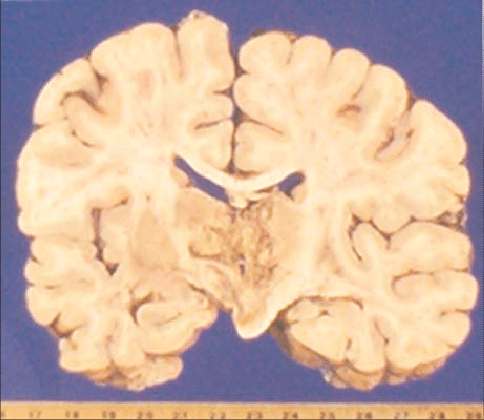
\includegraphics[width=0.75\linewidth]{chapters/introduccion/images/normal.jpg}
        \caption{Cerebro sano}
    \end{subfigure}
    \hspace{0.5cm}
    \begin{subfigure}[b]{0.45\linewidth}
        \centering
        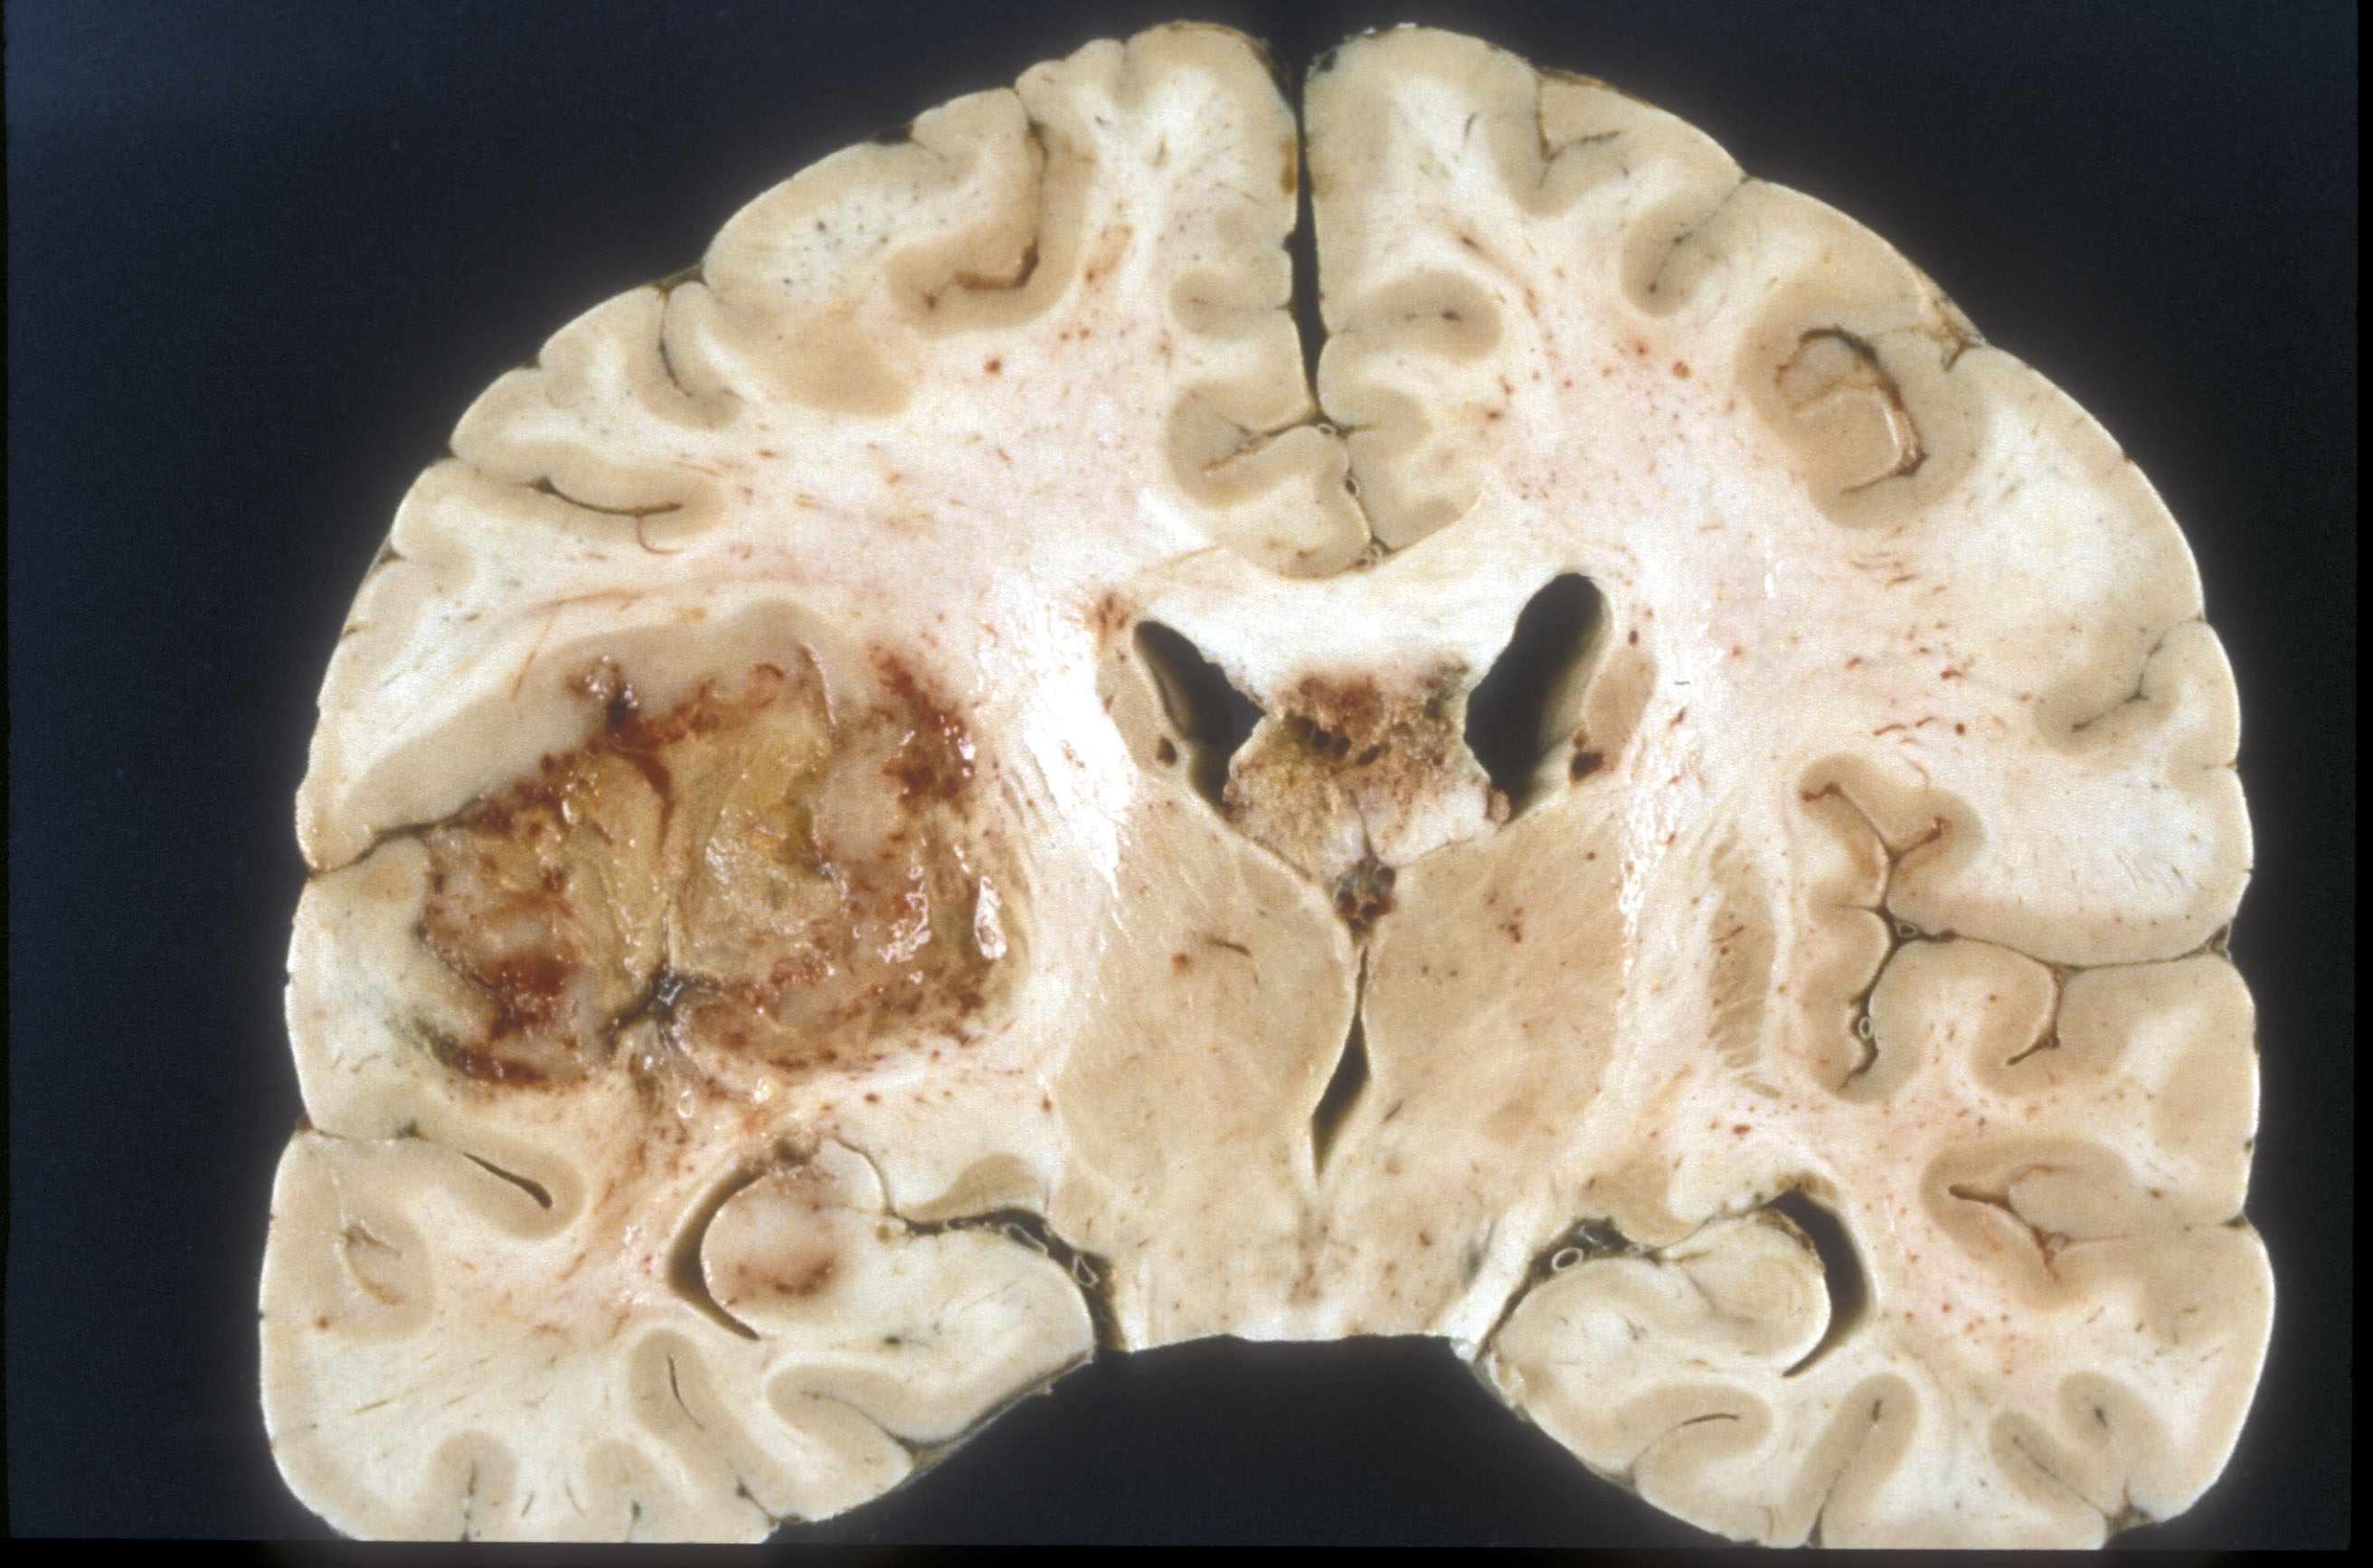
\includegraphics[width=\linewidth]{chapters/introduccion/images/tumor.jpg}
        \caption{Cerebro con tumor}
    \end{subfigure}
    \caption{Corte coronal de cerebro ex vivo sano y con un tumor.}
    \label{fig.cerebros}
\end{figure}

Los tumores cerebrales se pueden clasificar en primarios o secundarios, dependiendo de si se originan en el propio cerebro o se diseminan desde otra parte del cuerpo (también conocidos como metastásicos). Estas estructuras pueden variar en tamaño, donde algunos, incluso pequeños, pueden provocar síntomas graves y evidentes, mientras que otros de mayor tamaño pueden pasar desapercibidos debido a la falta de síntomas.

En términos generales, algunos tumores primarios son benignos, lo que significa que no son cancerosos. Sin embargo, con el tiempo, pueden crecer y afectar el tejido cerebral circundante al comprimirlo. Por el contrario, los tumores cancerosos pueden desarrollarse de manera rápida y agresiva, invadiendo y destruyendo el tejido cerebral sano a su alrededor.

\section{Motivación del trabajo}

La detección y segmentación de tumores cerebrales representan una tarea de gran importancia en el ámbito médico, según lo indicado por la Organización Mundial de la Salud (OMS). La capacidad de identificar y delimitar con precisión la ubicación y extensión de estos tumores es fundamental para la planificación de intervenciones quirúrgicas efectivas. La resección quirúrgica de los tumores cerebrales depende en gran medida de una detección temprana y una segmentación precisa, lo que puede significar la diferencia entre la vida y la muerte, así como entre la salud y la discapacidad permanente para los pacientes. Además, la detección oportuna de estos tumores permite iniciar el tratamiento adecuado en las etapas iniciales de la enfermedad, lo que puede mejorar significativamente los resultados clínicos y la calidad de vida de los pacientes al evitar complicaciones graves y preservar las funciones cerebrales vitales.

En este contexto, las técnicas de inteligencia artificial y aprendizaje profundo han emergido como herramientas poderosas y prometedoras. La aplicación de algoritmos de inteligencia artificial, como las redes neuronales convolucionales, permite procesar grandes volúmenes de datos de imágenes médicas de manera rápida y precisa, facilitando la identificación automática de características relevantes y la segmentación precisa de los tejidos tumorales. El uso de estas herramientas no solo agiliza el proceso de diagnóstico, sino que también mejora la precisión y fiabilidad de las predicciones, lo que puede conducir a una detección más temprana y un tratamiento más efectivo de los tumores cerebrales. En última instancia, la integración de la inteligencia artificial y las técnicas de aprendizaje profundo en la práctica clínica tiene el potencial de revolucionar el manejo de esta enfermedad, mejorando los resultados clínicos y la calidad de vida de los pacientes.

\section{Organización del Documento}

La organización del documento se estructura en dos partes principales. En la primera parte, se aborda la detección de tumores cerebrales, mientras que la segunda parte se centra en la segmentación de los mismos. Cada una de estas partes se desarrolla en un capítulo independiente, donde se discuten los fundamentos teóricos, las metodologías utilizadas y los resultados obtenidos en cada etapa del proceso.

Tras la presentación de los resultados, se procede a realizar un análisis detallado de las métricas correspondientes, evaluando la efectividad y precisión de los modelos desarrollados en la detección y segmentación de los tumores cerebrales. Este análisis se realiza con el objetivo de validar el rendimiento de los algoritmos y determinar su utilidad en la práctica clínica.

Finalmente, en el último capítulo del documento, se describe el diseño e implementación de una API y una página web interactiva sencilla. Estas herramientas permiten a los usuarios interactuar con los modelos desarrollados, facilitando su uso en entornos clínicos y de investigación. Se detallan las funcionalidades y características de la API y la página web, así como los pasos necesarios para su implementación y utilización efectiva.

Todos los detalles de código, armado de modelos, cálculo de métricas, procesamiento de datos, así como la implementación de la API y front end se encuentra en el \href{https://github.com/carlosng95/UCM-TFM}{Github}.






